\documentclass[
12pt,
english,
ngerman,
headsepline,
twoside,
openright,
numbers=noenddot,version=first
]{scrreprt}

\usepackage{lmodern}
\renewcommand{\sfdefault}{lmss}
\renewcommand{\ttdefault}{lmtt}
\usepackage[T1]{fontenc}
\usepackage[utf8]{inputenc}
\usepackage{listings}
\usepackage[a4paper]{geometry}
\geometry{verbose,tmargin=3cm,bmargin=3cm,lmargin=3cm,rmargin=2.75cm,headheight=1cm,headsep=0.666cm,footskip=1cm}
\setcounter{secnumdepth}{3}
\setcounter{tocdepth}{3}
\setlength{\parskip}{\medskipamount}
\setlength{\parindent}{0pt}

\usepackage{babel}

%% include jabref file
\usepackage{caption}
\usepackage{cite}
\usepackage{courier}
\usepackage{color}
\usepackage{emptypage}
\usepackage[usenames,dvipsnames,svgnames,table]{xcolor}
\usepackage{listings}
\usepackage[printonlyused]{acronym}
\usepackage{verbatim}
\usepackage{url}
\usepackage{graphicx}
\usepackage{setspace}
\usepackage{float}
\usepackage{graphicx}
\usepackage{subcaption}
\usepackage{color}
\usepackage{csquotes}
\usepackage{totcount}
\usepackage{csvsimple}
\usepackage{amsmath}
\usepackage{rotating}
\usepackage{adjustbox}
\usepackage{tabulary}
\usepackage{lscape}
\usepackage[nomargin,inline,marginclue,draft]{fixme}
%\usepackage{minted}
%\usepackage{fontspec}

\regtotcounter{chapter}

\setstretch{1.4}
\usepackage[unicode=true, 
 bookmarks=true,bookmarksnumbered=false,bookmarksopen=true,bookmarksopenlevel=2,
 breaklinks=false,pdfborder={0 0 0},backref=false,colorlinks=false]
 {hyperref}
\hypersetup{pdftitle={SAKWA},
 pdfauthor={Dragoljub Milasinovic}}
 
\makeatletter

% custom colors
\definecolor{lightergray}{gray}{0.95}
\definecolor{lighterergray}{gray}{0.98}

\DeclareCaptionFont{darkgray}{\color{darkgray}}
\DeclareCaptionFont{black}{\color{black}}
\DeclareCaptionFormat{listing}{\colorbox{lightergray}{\parbox{\textwidth}{#1#2#3}}}
\captionsetup[lstlisting]{font=sf,format=listing,margin=0pt,labelfont=darkgray,textfont=black}

\lstset{
	basicstyle=\scriptsize\ttfamily,
	tabsize=2,
	extendedchars=true,
	breaklines=true,
	frame=bt,
	framesep=4pt,	
    keywordstyle=\color{blue}\ttfamily,
	%keywordstyle=\color{violet}\bfseries,
    stringstyle=\color{red}\ttfamily,
	%stringstyle=\color{black}\ttfamily,
    commentstyle=\color{ForestGreen}\ttfamily,
	%commentstyle=\color{darkgray},    
	rulecolor=\color{lightergray},
	backgroundcolor=\color{lighterergray},
	showspaces=false,
	showtabs=false,
	xleftmargin=17pt,
	numbersep=5pt,
	numberstyle=\tiny,
	numbers=left,
	resetmargins=true,
	framexleftmargin=17pt,
	framexrightmargin=6pt,
	framexbottommargin=4pt,
	showstringspaces=false,
	morekeywords={__global__},
	columns=flexible
}

\lstloadlanguages{
	Java
}

% create css listing style
\lstdefinelanguage{JavaScript}{
  keywords={typeof, new, true, false, catch, function, return, null, catch, switch, var, if, in, while, do, else, case, break},
  keywordstyle=\color{blue}\bfseries,
  ndkeywords={class, export, boolean, throw, implements, import, this},
  ndkeywordstyle=\color{darkgray}\bfseries,
  identifierstyle=\color{black},
  sensitive=false,
  comment=[l]{//},
  morecomment=[s]{/*}{*/},
  commentstyle=\color{purple}\ttfamily,
  stringstyle=\color{red}\ttfamily,
  morestring=[b]',
  morestring=[b]"
}

\newcommand{\qq}{\symbol{34}} % 34 is the decimal ascii code for "
\newcommand\invisiblesection[1]{%
  \refstepcounter{section}%
  \addcontentsline{toc}{section}{\protect\numberline{\thesection}#1}%
  \sectionmark{#1}}


%%%%%%%%%%%%%%%%%%%%%%%%%%%%%% LyX specific LaTeX commands.
\providecommand{\LyX}{L\kern-.1667em\lower.25em\hbox{Y}\kern-.125emX\@}
%% Because html converters don't know tabularnewline
\providecommand{\tabularnewline}{\\}

%%%%%%%%%%%%%%%%%%%%%%%%%%%%%% Textclass specific LaTeX commands.
\newenvironment{lyxcode}
{\par\begin{list}{}{
\setlength{\rightmargin}{\leftmargin}
\setlength{\listparindent}{0pt}% needed for AMS classes
\raggedright
\setlength{\itemsep}{0pt}
\setlength{\parsep}{0pt}
\normalfont\ttfamily}%
 \item[]}
{\end{list}}

%%%%%%%%%%%%%%%%%%%%%%%%%%%%%% User specified LaTeX commands.
%% Flexibles Seitenlayout
\usepackage[automark]{scrpage2}

%% Mehrspaltenlayout ermöglichen
\usepackage{multicol}

%% Unterstützung für Farben
\usepackage{color}

%% Schönere Tabellen
\usepackage{booktabs, longtable}

%% Schönerer Blocksatz
\usepackage{microtype}

%% Mehr Platz zwischen Überschrift und Tabelle
\newcommand{\@ldtable}{}
\let\@ldtable\table
\renewcommand{\table}{ %
    \setlength{\@tempdima}{\abovecaptionskip} %
    \setlength{\abovecaptionskip}{\belowcaptionskip} %
    \setlength{\belowcaptionskip}{\@tempdima} %
    \@ldtable %
}

%% Verschiedene Symbole und Zeichen wie (c)
\usepackage{textcomp}

%% Deutsche Kurzfassung und englisches Abstract auf eine Seite
\renewenvironment{abstract}{
    \@beginparpenalty\@lowpenalty
        \begin{center}
            \normalfont\sectfont\nobreak\abstractname
        \end{center}
    \@endparpenalty\@M
}{
    \par
}

%% Alle Seiten vor dem Inhaltsverzeichnis sind römisch nummeriert
\pagenumbering{roman}
\let\myTOC\tableofcontents
\renewcommand\tableofcontents{
    \begin{spacing}{1.1}
    \myTOC
    \end{spacing}
    \clearpage
    \pagenumbering{arabic}
}

%% Kopfzeile um Logo ergänzen
\clearscrheadfoot
\ohead{\\\headmark}
\ihead{
\includegraphics[scale=0.4]{pics/2015_10_05_THB_Logo_BW}}%\pagemark}
\ofoot[\pagemark]{\pagemark}

%% Randnotizen anpassen
%\setlength{\marginparwidth}{22mm}
%\let \oldmarginpar = \marginpar
%\renewcommand{\marginpar}[1]{%
%    \-\oldmarginpar[\raggedleft\footnotesize\sf #1]%
%        {\raggedright\footnotesize\sf #1%
%    }}

%% Zitate am Kapitelanfang
\usepackage{epigraph}
\setlength{\epigraphwidth}{9cm}

\makeatother

\begin{document}
\titlepage

\begin{center}

\includegraphics[width=12cm]{pics/2015_10_05_THB_Logo_CMYK_randlos}\vspace{0.5cm}

\par\end{center}

\vspace{1cm}

\noindent \begin{center}
\textsf{\textbf{\large BACHELORARBEIT}}\textsf{}\\

\textsf{}\\
\textsf{\huge Serverless / Serverlose Architekturen für Konventionelle Webanwendungen}
\par\end{center}{\Large \par}

\vspace{2cm}

\noindent \begin{center}
{\huge }\begin{tabular}{rl}
Vorgelegt von: & Dragoljub Milasinovic\tabularnewline
Matrikelnummer: & 20140076\tabularnewline
am: & XX. Monat XXXX\tabularnewline
\end{tabular}
\par\end{center}{\huge \par}

\vspace{1cm}

\noindent \begin{center}
zum \\
Erlangen des akademischen Grades\textsf{}\\
\par\end{center}
\noindent \begin{center}
\textsf{\textbf{\large BACHELOR OF SCIENCE}}\textsf{\textbf{\LARGE }}\\
\textsf{\textbf{(B.Sc.)}}
\par\end{center}

\vspace{1cm}

\noindent \begin{center}
\medskip{}
\begin{tabular}{rl}
Erstbetreuer: & Prof. Dr.-Ing. Schafföner\tabularnewline
Zweitbetreuer: & Jonas Brüstel, M.Sc.\tabularnewline
\end{tabular}
\par\end{center}

\noindent \begin{center}
{\huge }
\par\end{center}{\huge \par}

\newpage{}

\selectlanguage{ngerman}%
\tableofcontents{}

\pagestyle{scrheadings}   

\chapter{Quellen}
Extending Moodle Functionalities with Ontology-based Competency Management
Ontology Suported Competency System
OpsWorks AWS :: Deployment Strategy
Cloud Design patterns :: Profi Patterns
Man Trade Offs Arch :: Auswertung + Design guide  <- self-adaptive arch?? 
AWS Sol. Arch :: Best Practices AWS vs Patterns general 
Amazon Web Services in Action :: Best Practices Arch
Impl Cloud Design-Patterns for AWS :: Patterns list
Serverless Arch AWS :: Main :: lambda: compute as a back end 


\chapter{Einleitung}{Idee-Ausführung-Markt}
\setcounter{page}{1}
\label{chap:introduction}
\epigraph{\textit{\textquotedbl{}
		An idea is not a mockup\\
		A mockup is not a prototype\\
		A prototype is not a program\\
		A program is not a product\\
		A product is not a business\\
		And a business is not profits.\textquotedbl{}}}{
	Balaji S. Srinivasan }


Die vorantreibende Aspekte solcher Zustandsmaschine sind die Ausführung/Umsetzung der Idee bis zum Produkt und derer Beziehung zum Markt. Deren Details sind jedoch unbekannt und variabel. 

Die Faktoren am Anfang einer technologischen Umsetzung einer Idee sind: 
Time-To-Market
Kost of Human Resources:: Skill shortage
Prof of Concept
Technical technological details
Profitability


\section{Motivation}


Auf dem Weg zur technologischen Umsetzung einer neuen Idee liegen unbekannte Schwierigkeiten
bei der Entscheidungen über die Architektur der Anwendung/Projekt/Umsetzung?,
der Drittanbieter von Software, der Auswahl der Infrastruktur usw.
Schwierigkeiten die von spezialisierten Kompetenzen, Fertigkeiten und \glqq Know-How\grqq bedürfen.
Gehören jedoch nicht immer zum Problem des Domäns der Anwendung.

Um sich von diesem spezialisierten wissen aufzulösen wurde ...

Für dieses Problem wurde \glqq FaaS\grqq als Lösung unter der Rubrik \glqq Serverless\grqq von den Hauptanbieter von \glqq Cloud\grqq Technologien vorgestellt.

Im Rahmen des Cloud-Computing handelt es in dieser Arbeit um eine Untersuchung der Serverless Architekturen am Beispiel einer Konventionellen Webanwendung. Dabei wird besonders geachtet ob und wie solche Technologien die Umsetzung erleichtern. Die Entwurfsmuster und die Kernfunktionalität werden mit ausschließlich Serverless Technologien am Beispiel von KOMA mit AWS umgesetzt.


\section{Ziel}
\label{sec:task}


@acronym MVP Minimal Viable Product : \cite{rady2016serverless}
Als Ergebnis wird ein MVP Minimal Viable Product in form eine @acronym SPA Single Page Application vor zur Verfügung gestellt.

Start::Chars: Arch + Domän Flexibilität - Schnelle Arch Änderungen

Umsetzung der Kernfunktionalität einer Beispielanwendung mit ausschließlich \glqq Serverlosen\grqq Architekturen.
wenn Zeit: Identifizieren von unverzichtbare Generische Funktionen für Serverless Anwendungen.
%Identify Generic Functions with-/out Architecture Pattern


\section{Aufbau der Arbeit}
\label{sec:layout}

Zuerst wird den Leser in die Serverless \ref{sec:serverless} Technologien eingeführt, das Programmiermodell vorgestellt
und die Entscheidungsprinzipien erläutert.
%Als Zweites wird KOMA \ref{sec:KOMA} als vorläufiges Beispielanwendung und deren Anforderungen vorgestellt.<-- nice to have
Eine Zahl von möglichen Kombinationen von aktuellen Technologien mit Serverless werden beispielhaft dargestellt.
Hinzu wird derer Analyse und Umsetzung durchgeführt und erläutert.

\chapter{Grundlagen}
\label{chap:principles}

Serverless ist ein @Glossar Web Dienst/Service von Cloud-Anbieter, wird auch als @Glossar FaaS bezeichnet. Deren Serverinfrastruktur wird vom Cloud-Anbieter wie Amazon Web Services verwaltet. Komplexe Probleme wie horizontale und vertikale Skalierbarkeit, Fehlertoleranz, Flexibilität werden von Kunden nur noch nach bedarf Konfiguriert. 


\section{Serverless}
\label{sec:serverless}
Prinzipien von Serverless Architeturen: \cite{sbarski2017serverless}
Rechen-Dienst nach Anfrage dass in isoliert, unabhängig und granular ausgeführt wird. 
. . .



Programmiermodell 
Dienste werden nach Anfrage ausgeführt. 
Die Kosten werden nach Ausführung abgerechnet. 

One size fits NOT all

Vergleich mit Microservices.


Stand der Technik: 
Vorgehensweise bei Traditionelle Webanwendungen:  
Software Architektur: "What's important". Frühe, un-/schwer- veränderbare Entscheidungen.
%@Glossar: 
Web Services are processes that expose their interfaces to the Web so that users can invoke them. Facilitate service discovery and meaning encoded in schemas


Design: Lambda Orchestrator -> Pool of Lambdas to use

\section{KOMA}{Beispiel Anwendung}
\label{sec:KOMA}

Die heutige Rahmenlehrpläne sind nicht mehr fachlich sondern kompetenz orientiert. @cite Deren ziel ist Kompetenzprofile
für Lerner zu gestallten. Das Modell von KOMA basiert auf dem Grundmodell von
@ref \glqq European Qualifications Framework Semantics\grqq und dem deutschen Qualifikationsrahmen. <-- really?

\glqq KOMA\grqq ist ein Akronym für Kompetenz-Matrix. Die Umsetzung der Anwendung soll die von einem Individuum oder Schuler
erworbene und zu erwerbenden Kompetenzen und deren Niveau nachvollziehen. <-- ?
Der Kompetenzstand einer Person ist mit dem EQF-Rahmen @Acro vergleichbar, und daher Internationell anerkenntbar.
%Diese soll für die pädagogische Diagnostik und Intervention genutzt werden.
Wenn diese Anwendung in Bildungsintitutionen eingesetzt wird, dienen die Rahmenlehrpläne als Leitpfad für die Belegung der einzelnen Kompetenzen
und KOMA für die Organisation der einzelnen Fachrichtungen. Der Kern solcher Org. ist die Zuweisung von Aktivitäten auf vordefinierten Kompetenzen.
Aktivitäten lassen sich einzeln oder in einer Sequenz anordnen. Sequenzen werden in LVen zusammengestellt. So können Aktivitäten, Sequenzen und Kompetenzen
als gestalltungsmittel für LV benutzt. Das Modell verfügt von eine Figur um die erledigte Aktivitäten auszuwerten, nämlich Evaluation.

Wegen der Kompetenzorientierung, wird Kompetenz als Unit-Of-Work betrachtet für Modelierungszwecke.

Beispiel:
Der Lehrplan fordert die Kompetenzen K in K1, K2, K3 .. Kn für den Bachelordiplom. Nach deren Manuellen Eingabe werden automatisch
ihren Requirenments/Abhängigkeiten Baum erzeugt. Dadurch können bereiche des Baums als LV betrachtet werden und Kompetenzen aufeinander
bauend für eine Klassenstufe/Semestergang sequenziert werden. Die Auswertung der Ergebnisse der Aktivitäten und die Aktualisierung des Kompetenzstands
des Schulers folgen.

Ein Nutzungs-Fall aka. Use-Case: 
-Als Professor, will ich eine Auflistung der erworbene Fertigkeiten einer Klassenstufe abrufen können.

-Als Professor, will ich das Kompetenzniveau einer Kompetenz eines Studenten und deren Fertigkeiten abrufen können.

-Als Student, will ich mein Kompetenzprofil für meinen Lebenslauf benutzen.

\chapter{Umsetzung}
Die grundlegende Vorgehensweise bei der Umsetzung dieses Projekts wird Analyse, Entwurf, Implementierung und Test sein. Der Forschender Charakter dieses Projekts lässt sich nicht Testgetrieben zu implementieren. 

\section{Komponenten}

@Diagramm

\section{Anforderungen Analyse}
Mit dem EQF vergleichbare Kompetenzendefinitionen.

Von Browser abrufbar. 

Private Datenspeicherung. Daher Login.

Zukünftige Erweiterungen berücksichtigen.

\section{Serverless Kombiniert}
Spring Boot + Lambda
Wildfly Swarm REST + Lambda
Django + Lambda

\section{Datenhaltung Analyse und Auswahl}


%@Pre-Dev--> Tabelle 
Vergleich:: DB Schema                       : Ontology
Welt-Annahme Existiert nur Abbild           : mindestens Abbild
Individual=Instanz muss unique              : kann >= 1
Info Ableitung = x                          : ja
Oritentation    Data                        : Bedeutung

%@Pre-Dev::Feasibility Study
Es wurden folgende Faktoren für die Entwicklung einer Ontologie erkannt:
%@list
Zirkuläre Abhängigkeiten sind zugelassen.  
Equivalenzklassen zwischen KOMA und andere Ontologie soll die Anerkennung von erworbenen Kompetenzen ermöglichen.
Die Begriffe der Kompetenzen können sich ändern oder die Ontologie soll erweitert werden.
Die Verbindung zu externen Ontologien kann neues Wissen ableiten.
6.2.2 \cite{OntoCloud}Benefits on Interoperability and Linked-Data by Using
Ontology Engineering

\subsection{Ontologie}

Das \glqq Semantic Web\grqq ist eine Erweiterung des herkömmlichen Web, in der Informationen mit eindeutigen Bedeutungen versehen werden@Cite. Diese Bedeutungen wirden für Maschinen durch Ontologien dargestellt. Die Ontologien werden in der OWL2 Spezifikation von W3C@Ref beschrieben. 
%@Def
Eine Ontologie ist eine Darstellung von Wissen. Präziser: eine formale Spezifikation über eine Konzeptualisierung\cite{OntoWhat}.
%@Cite :  R. Studer, R. Benjamins, and D. Fensel. Knowledge engineering: Principles andmethods.Data & Knowledge Engineering, 25(1–2):161–198, 1998
Während der Umsetzung wurde Protege\footnote{\url{http://protege.stanford.edu}: "This work was conducted using the Protégé resource, which is supported by grant GM10331601 from the National Institute of General Medical Sciences of the United States National Institutes of Health."} benutzt.
Der Entwurf der Ontologie wurde nach Ontology-Engineering-101
 durchgefuhrt: 
%@Citehttps://protege.stanford.edu/publications/ontology_development/ontology101-noy-mcguinness.html

%@Pre-Dev::Environ

Software platform ? 
Die Clients : REST: sparql Endpoints

Die Daten werden in Produktion @Anglizismus in einer \glqq Triple-Store\grqq mit grundsätzlich 4 alternativen: Monolitische Triple Speicherung, Property Werte, Vertikal Partitionierte Tables und Hexastore @Cite hpi web-sem 2.9. 
Als Ansatz eignet sich S3 @Acro für die Speicherung von großen Datenmengen. Der nächste Schritt wird eine Indexierung der URIs jeweiliger Subject, Predicate und Object in DynamoDB @Acro .

Der Zugriff auf die Ontologie wird direkt mithilfe von \glqq SPARQL\grqq  realisiert. Deren Quelldateien werden in einer Lambda @Acro ausgeführt.

ontol-eng 101
1-determine-scope: 
Die Verwaltung von Fortschritten der Studierenden im Kompetenzrahmen der Lehrpläne.

%2-Consider reuse: 
Obwohl die LOD @Acro NNN Datebasis erkannt hat und Watson @Cite Begriffe wie Kompetenz in zahlreiche Ontologien gefunden hat, konnte ich einen aktuell öffentlichen graphischen Entwurf\cite{OntoMoodle} @Cite onto-moodle einer Ontologie finden. 
%@Bild onto-moodle
Bei der Analyse lässt der Entwurf und dessen Dokumentation freie Interpretation über Begriffe und deren Zweck bzw. bie \glqq isComposedOf\grqq, \glqq subsumes\grqq. Ein Standard zur graphischen Darstellung ist zur Zeit?? noch nicht anerkannt.@Cite research-gate graphol

Anderseits wurde ein \glqq EQF Framework\grqq für Ontologien beschrieben, aber nicht öffentlich umgesetzt. Es bietet dabei eine europäisch anerkannte Definition von Kompetenz, nämlich RCD @Acro.

Daher folgt eine beispielhafte Enumeration der auf unseren Anwendungsfall angepasste und ergänzende Interpretation der dargestellten Terminologie des Entwurfs und der RCD.
%@pic: own mix for both

%3-Enumerate Terms:  Terminologie
Nur Beispielhaft
\begin{table}[H]
	\caption{Terminologie}
	
	
	\noindent \centering{}\begin{tabular}{ccc}
		\hline 
		\noalign{\vskip\doublerulesep}
		Darstellung & Begriff & Bedeutung\tabularnewline[\doublerulesep]
		\hline
		\noalign{\vskip\doublerulesep}
		Competence & Kompetenz & Kontext adäquate Anwendung von Fertigkeiten \tabularnewline[\doublerulesep]
		\noalign{\vskip\doublerulesep}
		CompetenceProfile & Kompetenzprofil & Sammlung von Kompetenzen \tabularnewline[\doublerulesep]
		\noalign{\vskip\doublerulesep}
		Competence & Kompetenz & Kontext adäquate Anwendung von Fertigkeiten \tabularnewline[\doublerulesep]
		\noalign{\vskip\doublerulesep}
		Skill & Fertigkeit & Das systematisch Tun-Können einer Aufgabe \tabularnewline[\doublerulesep]
		\noalign{\vskip\doublerulesep}
		Knowledge & Wissen & Verstehen von Informationen
		\tabularnewline[\doublerulesep]
		\noalign{\vskip\doublerulesep}
		Other & Andere & Nicht kategorisiert aber zu beachten
		\tabularnewline[\doublerulesep]
		\noalign{\vskip\doublerulesep}
		ProficiencyLevel & Kompetenzniveau & Bewertung einer Kompetenz
		\tabularnewline[\doublerulesep]
		\noalign{\vskip\doublerulesep}
		PerformanceIndicator & Kompetenzmaß & Kriteria zur Auswertung
		\tabularnewline[\doublerulesep]
		\noalign{\vskip\doublerulesep}
		Course|LV & Lehrveranstaltung & Sammlung von Sequenzen
		\tabularnewline[\doublerulesep]
		\noalign{\vskip\doublerulesep}
		Sequenz & Sequenz & Sammlung von Aktivitäten
		\tabularnewline[\doublerulesep]
		\noalign{\vskip\doublerulesep}
		Activity & Aktivität & Lernaktivität
		\tabularnewline[\doublerulesep]
		\noalign{\vskip\doublerulesep}
		Action & Aktion & Lerntat
		\tabularnewline[\doublerulesep]
		\noalign{\vskip\doublerulesep}
		Actor & Täter & Aktiver Agent aka Lerner
		\tabularnewline[\doublerulesep]
		\noalign{\vskip\doublerulesep}
		Learner & Lerner & Kompetenz erwerbender Agent
		\tabularnewline[\doublerulesep]
		\noalign{\vskip\doublerulesep}
		CompetencyRecord & Kompetenzaufnahme & --
		\tabularnewline[\doublerulesep]
		\noalign{\vskip\doublerulesep}
		EvidenceRecord & Kompetenzbeweis & --
		\tabularnewline[\doublerulesep]
		\noalign{\vskip\doublerulesep}
		EvidenceSource & Kompetenzherkunft & --
		\tabularnewline[\doublerulesep]
		\noalign{\vskip\doublerulesep}
		todo & todo & todo
		\tabularnewline[\doublerulesep]
		\noalign{\vskip\doublerulesep}
		todo & todo & todo
		\tabularnewline[\doublerulesep]
		\hline
	\end{tabular}
\end{table}


4-Define Classes and Hierarchies:
Um Wissen abzuleiten und Inkonsistenzen zu identifizieren werden die Klassen und Properties durch Restrictions versehen oder definiert. Folgende Restrictions wurden angewendet. 
\begin{table}[H]
	\caption{Klassendefinition}
	
	\noindent \centering{}\begin{tabular}{cc}
		\hline 
		\noalign{\vskip\doublerulesep}
		Klasse & Definition \tabularnewline[\doublerulesep]
		\noalign{\vskip\doublerulesep}
		LV & only Sequenz \tabularnewline[\doublerulesep]
	\end{tabular}
\end{table}


Alle Klassen in einer Ontologie leiten sich von \glqq owl:Thing\grqq. ?? 
Skill skos:Concept @Ref
@Build : ableitungs Baum von Protege

5-Define Properties/Attributes of Classes: 
\begin{table}[H]
	\caption{Properties}
	
	\noindent \centering{}\begin{tabular}{cc}
		\hline 
		\noalign{\vskip\doublerulesep}
		isComposedOf & $\forall{Class} \equiv only Class$ \tabularnewline[\doublerulesep]
		\noalign{\vskip\doublerulesep}
		subsumes & $\exists{Class} \equiv some Class$ \tabularnewline[\doublerulesep]
	\end{tabular}
\end{table}


ontol- engineering for methodology 
types : top - domain - app
semantic gap:: how to find out whether 2 ontologies mean the same thing
ontologies enable interoperability of metadata: 
design for develop
mapping for comparison
merging for efficient combination of ontologies
learning for learn new ontos from given sets

desing: 
activities: management - develop - support
management
scheduling - control - quality assurance
development
pre - develop - post
suport
knowledge acquisition - eval - integr - merge - align->map - doc - config man

design:app
Konkrete Fragestellungen für die pädagogische Diagnostik und Intervention.

welche stand von kompetenzen hat eine Klassenstufe?
kompetenz-rückstände/auffälligkeit von eine Klassenstufe?
gegeben sein ein stand, welche leistung kann ich von Klassenstufe erwarten?
wurde skill-x zu Klassenstuf-y vergeben? 

\section{Repository}

Um aus Ontologien Informationen zu entnehmen, wird die Abfragesprache \glqq SPARQL\grqq @Acro verwendet. Diese ist ähnlich zu SQL. Mit dem Programm \glqq Protétegé\grqq können SPARQL Abfragen lokal ausgeführt werden. 
@Bild Protege SPARQL query

So dass auch die Benutzer von KOMA solche Abfragen stellen können wird ein \glqq Sparqlendpoint\grqq mit Hilfe von Apache Jena Fuseki@Cite, eine Open Source Software, zur Verfügung gestellt. Fuseki ist ein Server zur Verwaltung von Sparqlabfragen und deren Transaktionen. @Cite CRUD und ACID RDB in sparql. 

@First Serverless Info
Fuseki wird Embedded benutzt.
Fuseki entspricht der Repositoryschicht der Anwendung und wird nach Anfrage von der Ontologie in S3 mittels Sparql JSON Objekte zurückliefern. 
Eine Lambdafunktion arbeitet als Schnittstelle zwischen Fuseki, den Client und die darunterliegende Infrastruktur. 

Um sich von die durch Lambda entstandene Abhängigkeit möglichst entkoppelt\cite{FlowerRefactoring} zu halten, wird das Modul von Fuseki nur als externe Abhängigkeit des Lambdaprojektes zugewisen. 
@Code : Gradle build\cite{Muschko2014}

RESTful API \\
Unter der verfügbaren SparQL endpoints Implementierungen

Methode http://<host>/ontology/entity -> meta-info über Ontologie

http://www.example.com/id/alice
Identifier for Alice, the person
http://www.example.com/people/alice
Alice's homepage
http://www.example.com/data/alice
RDF document with description of Alice

\section{UI-IT}

Die Benutzeroberfläche soll im Browser realisiert werden. Initializr bietet die Erstellung einer konfigurierten Projektstruktur an. Es wird NodeJS als Laufzeitumgebung, NPM als Packetmanager, Bootstrap als Stylescheet und jQuery als Javascript-Bibliothek benutzt. 

Grund weshalb Statisch und S3:: 

Die Webseite wird Statisch mittels S3 geliefert. Da der Zugriff auf die Datenspeicherung gesichert werden soll, wird die  Login-Funktionalität hinzugefügt.@Ref Einloggen
@Code webify bucket



\section{Einloggen}

Autorisierung und Authentifizierung. Einleitung

Auth0 bietet Authentifizierung as a Service an. Mit wenige Konfigurationsschritte kann man die Benutzer Authentifizieren. 


Einloggen: 0Auth Google gibt token, der wird in Lambda überprüft, Session in oauth.com verwaltet
Query: SparQL ?x, ?y, ?z WHERE ...
Datenspecherung Architektur:
DynamoDB: speichert :individual als Schlussel und seine relative URL
Ś3: speichert die .owl Dateien.

Lambda Funktion: Maps zwischen S3 und DynamoDB.

\section{Patterns}

Die Architekturentwurfsmuster helfen uns zu kommunizieren welches Zweck unsere Software erreichen möchte und bieten generische Lösungen für wiederkehrende Probleme bei der Softwareentwicklung.

Tier vs Layer: \cite{sbarski2017serverless}

Separation of concerns
Reusable layers
Maintenance @Schafföner JEE1

Components: 
Controller: router, handle in-req build out-res
Service: @Transaction
Repository: 1-1 mapping to db

Wenn eine erfolgreiche Codeänderung von andere Änderung abhängt, soll die Architektur überprüft werden. 

Valet Key \cite{homer2014cloud}

Static Content Hosting ok

Sharding ok

Compute Resource Consolidation 

Command and Query Responsability Segregation CQRS <- readS3UpdateDynamo.js

\chapter{Ergebnis und Auswertung}
Vorteile

Automatische Skalierung und Fehlertoleranz
Automatisches Kapazitätsmanagement
Flexible Ressourcenverwaltung
Schnelle Bereitstellung der Ressourcen
Exakte nutzungsabhängige Abrechnung der Ressourcen
Konzentration auf den Kern des Source-Codes
Nachteile:

Kontrollverlust
Erhöhtes Lock-in Risiko

kurzlebige konfigurationen herausfinden ?? tracking?
viel Konfiguration, kaum Konveniton -> .json 4 everything
local testing braucht event-symulation.json

\chapter{Zusammenfassung und Ausblick}


Beispielhaftes Bild \autoref{fig:example-flame-graph}

\begin{figure}[h]
	\centering
	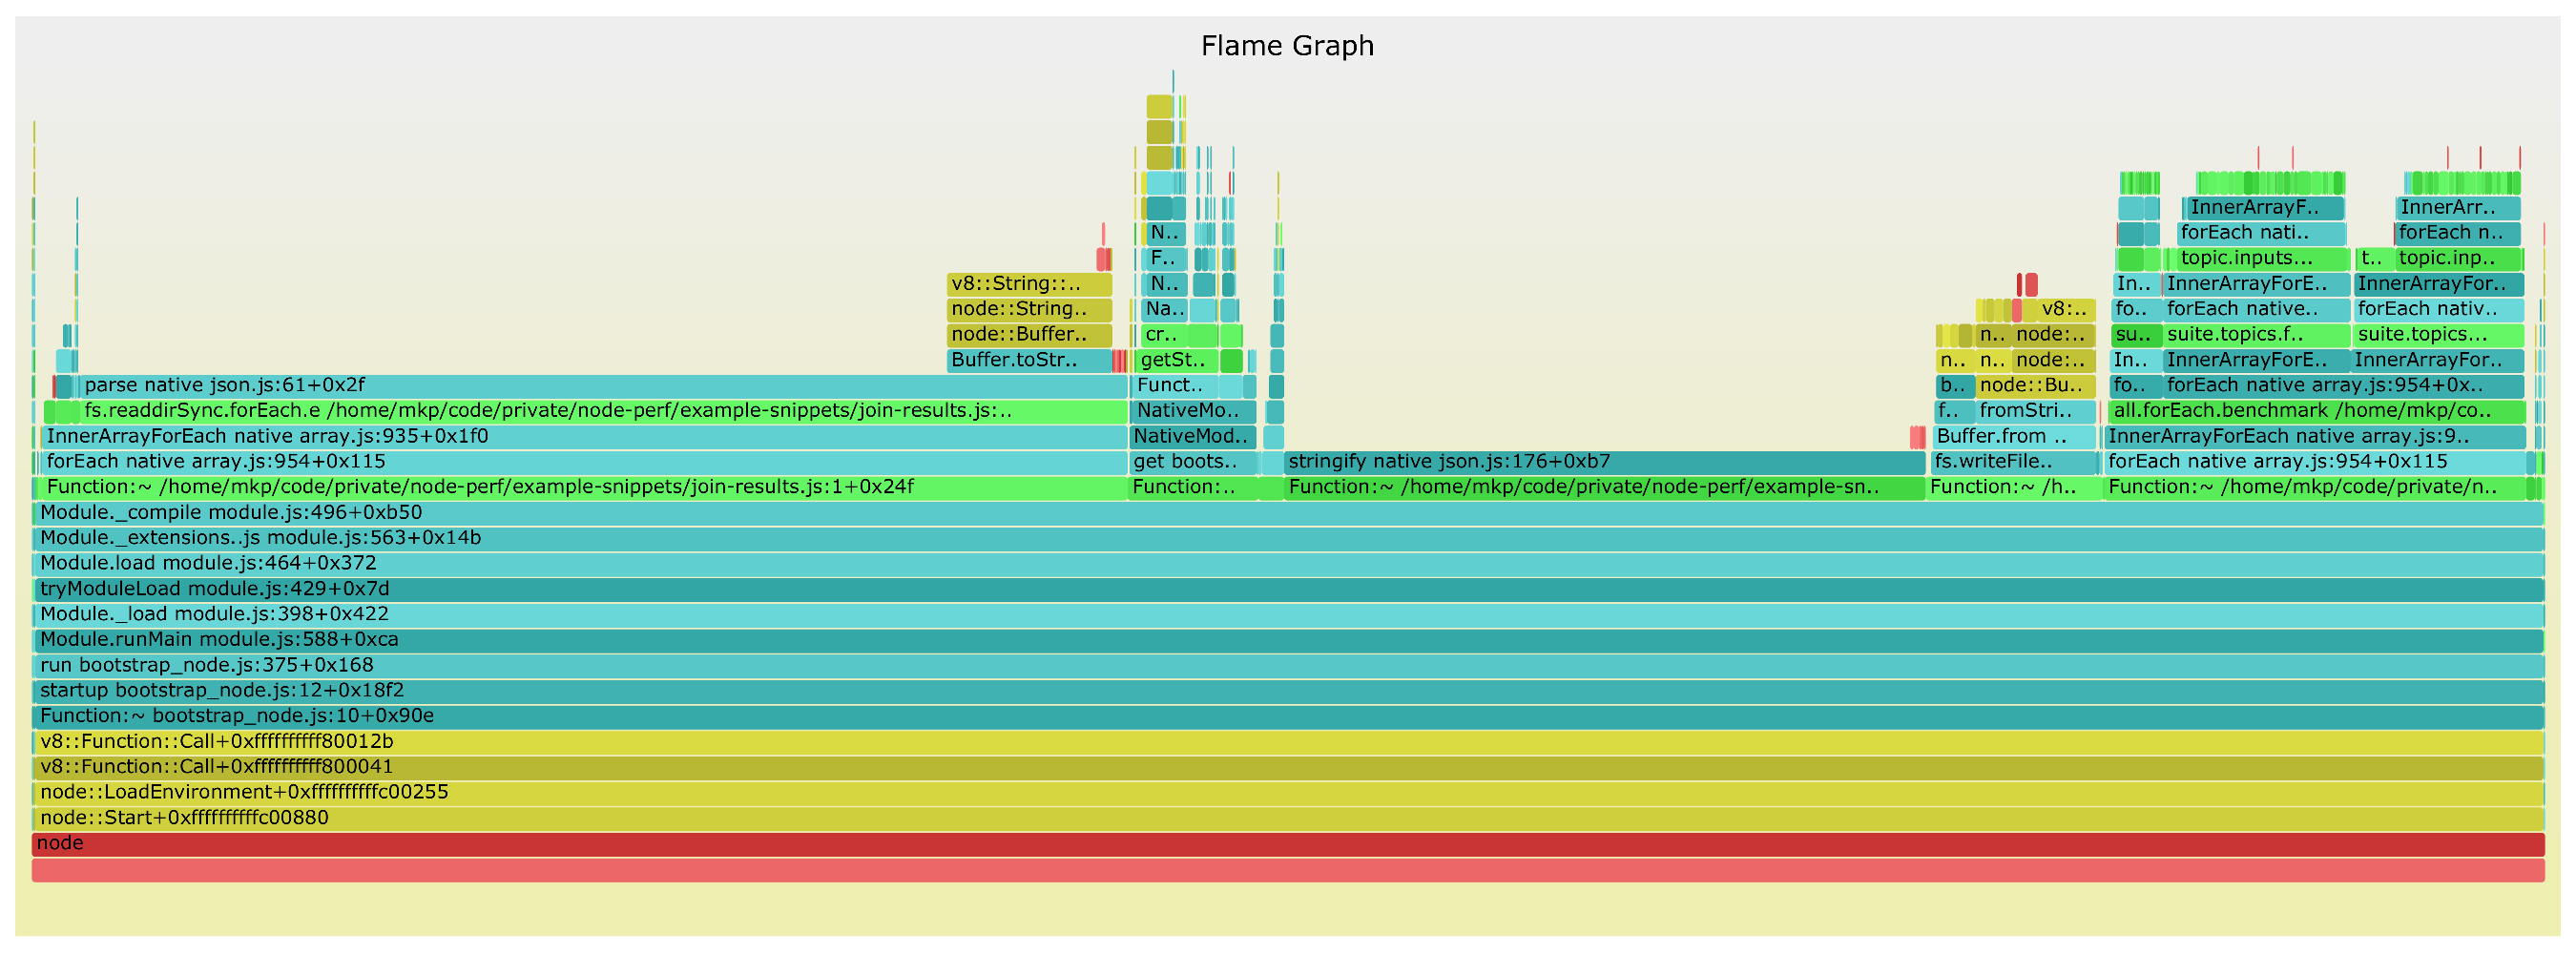
\includegraphics[width=0.8\textwidth]{pics/example-flame-graph.eps}
	\caption{Beispiel Flame-Graph eines Node.js Skripts}
	\label{fig:example-flame-graph}
\end{figure}

Beispielhaftes Code-Snippet siehe \autoref{lst:sample}.

\begin{lstlisting}[language=bash,caption={Aufnahme der \glqq real\grqq-Zeit},label={lst:sample}]
START=$(date +%s.%N)
node ${JS_FILE}
END=$(date +%s.%N)
DIFF=$(echo "$END - $START" | bc)
\end{lstlisting}

Hier kommt eine Bibliography-Referenz: \cite{booch2007object}

\lstlistoflistings

\listoffigures

\listoftables

\chapter*{Abkürzungen}
\markboth{Abkürzungen}{}

%@Glossar
%ontology: explicit, formal specification of a shared conceptualization
%Semantic Gap: Diferent ontologies to representate/ describe the same thing
%Polisemy ptoblem

%Formale Darstellung von Wissen durch eine Menge von Konzepten innerhalb eines Domänes und dessen Beziehungen -zwischen Konzepten-. way to mix together different descriptive vocabularies in a consistent way. Vocabularies can be created by distinct communities and groups as appropriate and mixed together as required, without needing any centralized agreement on how terms from different vocabularies can be written down in XM


%p.6 Studies in computational intlligen Ontologies: Level 4 SaaS :Scalable, Configurable, and Multitenant

%https://de.slideshare.net/UscholdM/ontologies-and-db-schema-whats-the-difference
%https://www.youtube.com/watch?v=bGPVCkuKTo4
%https://www.youtube.com/watch?v=n1hwsclr0Eg

%https://db-engines.com/de/system/Amazon+DynamoDB;GRAKN.AI;H2
%https://stackoverflow.com/questions/36255919/can-i-use-an-ontology-as-database-and-store-data-within-it

%nosql: https://de.wikipedia.org/wiki/NoSQL

%@Glossar
%Semantics: relationships between signifiers
%De-notation: precise literal meaning of signifier
%Con-notation: associated meanings of signifier


\begin{acronym}[Bash]
	

\acro{GC}{Garbage Collection}

\glqq Garbage Collection\grqq{} bezeichnet die automatische Speicherwaltung zur Minimierung des Speicherbedarfes eines Programmes.
\ac{GC} wird zur Laufzeit durch Identifikation von nicht mehr benötigten Speicherbereichen ausgeführt.
Im Vergleich zur manuellen Speicherverwaltung benötigt \ac{GC} mehr Ressourcen.

\end{acronym}

\bibliographystyle{alpha}
\bibliography{sources}


\chapter*{Eidesstattliche Erklärung}

Ich versichere hiermit, dass ich die von mir eingereichte Masterarbeit selbstständig verfasst, ausschließlich die angegebenen Hilfsmittel benutzt und sowohl wörtliche, als auch sinngemäße entlehnte Stellen als solche kenntlich gemacht habe. Die Arbeit hat in gleicher oder ähnlicher Form noch keiner anderen Prüfungsbehörde vorgelegen.

Brandenburg an der Havel, XX. Monat 2017

\vspace{3cm}

Vorname Nachname

\end{document}
